%%%%%%%%%%%%%%%%%%%%%%%%%%%%%%%%%%%%%%%%%%%%%%%%%%%%%%%%%%%
\documentclass[xcolor=x11names,compress]{beamer}
%\documentclass[xcolor=x11names,compress, handhouts, aspectratio=169]{beamer}
%% General document
\usepackage{graphicx, subfig}
%% Beamer Layout
\useoutertheme[subsection=false,shadow]{miniframes}
\useinnertheme{default}
\usefonttheme{serif}
\usepackage{palatino}

%%%%%%% Mes Packages %%%%%%%%%%%%%%%%
%\usepackage[french]{babel}
\usepackage[T1]{fontenc}
\usepackage{color}
\usepackage{xcolor}
\usepackage{dsfont} % Pour indicatrice
\usepackage{url}
\usepackage{multirow}
\usepackage[normalem]{ulem}   % For strike out text

% Natbib for clean bibliography
\usepackage[comma,authoryear]{natbib}

%remove the icon
\setbeamertemplate{bibliography item}{}

%remove line breaks
\setbeamertemplate{bibliography entry title}{}
\setbeamertemplate{bibliography entry location}{}
\setbeamertemplate{bibliography entry note}{}

%% ------ MEs couleurs --------
\definecolor{vert}{rgb}{0.1,0.7,0.2}
\definecolor{brique}{rgb}{0.7,0.16,0.16}
\definecolor{gris}{rgb}{0.7, 0.75, 0.71}
\definecolor{twitterblue}{rgb}{0, 0.42, 0.58}
\definecolor{airforceblue}{rgb}{0.36, 0.54, 0.66}
\definecolor{siap}{RGB}{3,133, 200}


%%%%%%%%%%%%%%%%% BEAMER PACKAGE %%%%%%%

\setbeamercolor{itemize item}{fg=siap}
%\setbeamercolor{itemize subitem}{fg=blue}
%\setbeamercolor{itemize subsubitem}{fg=cyan}

\setbeamerfont{title like}{shape=\scshape}
\setbeamerfont{frametitle}{shape=\scshape}

\setbeamercolor*{lower separation line head}{bg=DeepSkyBlue4}
\setbeamercolor*{normal text}{fg=black,bg=white}
\setbeamercolor*{alerted text}{fg=siap}
\setbeamercolor*{example text}{fg=black}
\setbeamercolor*{structure}{fg=black}
\setbeamercolor*{palette tertiary}{fg=black,bg=black!10}
\setbeamercolor*{palette quaternary}{fg=black,bg=black!10}

% Set the header color to SIAP's color
\setbeamercolor*{frametitle}{fg=siap}

%remove navigation symbols
\setbeamertemplate{navigation symbols}{}

\renewcommand{\(}{\begin{columns}}
\renewcommand{\)}{\end{columns}}
\newcommand{\<}[1]{\begin{column}{#1}}
\renewcommand{\>}{\end{column}}

%% Add footer with logo
\setbeamertemplate{footline}{%
  \begin{beamercolorbox}[wd=\paperwidth,ht=2.5ex,dp=1.125ex,%
    leftskip=.3cm,rightskip=.3cm plus1fil]{author in head/foot}
    \includegraphics[height=4ex]{SIAP_logo_Big.png}\hfill
    \insertshortauthor\hfill\insertshorttitle\hfill  \textcolor{siap}{\textit{\insertframenumber}}
  \end{beamercolorbox}%
}

% Path for the graphs
\graphicspath{
{Graphics/}
{c:/Chris/UN-ESCAP/SIAP-E-learning/Resources/OpenScience/}
{c:/Chris/Visualisation/Presentations/Graphics/}
{c:/Chris/Visualisation/Presentations/Graphics/SIAP/}
{c:/Chris/Visualisation/Presentations/Graphics/Lies/}
{c:/Chris/Visualisation/Presentations/Graphics/Maps/}
{c:/Chris/Visualisation/Presentations/Graphics/RGenerated/}
{c:/Chris/Visualisation/Presentations/Graphics/Logos/}
{c:/Gitmain/MLCourse/UNML/Module0/M0_files/figure-html/}
{c:/Chris/UN-ESCAP/MyCourses2022/MLOS2022/Slides/Graphics/}
{c:/Chris/UN-ESCAP/MyCourses2023/RAP/Slides/Graphics/}
{c:/GitMain/RAP/RAP-Course/images/}
{c:/Chris/UN-ESCAP/MyCourses2022/MLOS2022/Slides/Graphics/}
% Path for specific graphs created
 {../R-Codes/JobSatisfaction_files/figure-latex/}
 {../R-Codes/Unused_files/figure-latex/}
 }


\title{\textcolor{siap}{JICA-TAPOS}}
\subtitle{\textcolor{siap}{\large{Data Visualization - Descriptive \& Inferential  Statistics}}}
\author{Christophe Bontemps}
\institute{\large{\emph{Statistical Institute for Asia and the Pacific} } \\
    \includegraphics[height=10ex]{SIAP_logo_Big.png}}
\date{}


\begin{document}

\begin{frame}
  \titlepage
\end{frame}

\begin{frame}{Fundamental Principles of Official Statistics}
  \begin{columns}[T]
    \begin{column}{0.6\textwidth}
      \begin{itemize}
        \item Clear mention of the process used to produce statistics
        \item To retain trust in official statistics, the statistical agencies need to decide according to strictly professional considerations, including scientific principles and professional ethics, on the methods and procedures for the collection, processing, storage and presentation of statistical data.
      \end{itemize}
    \end{column}
    \begin{column}{0.4\textwidth}
      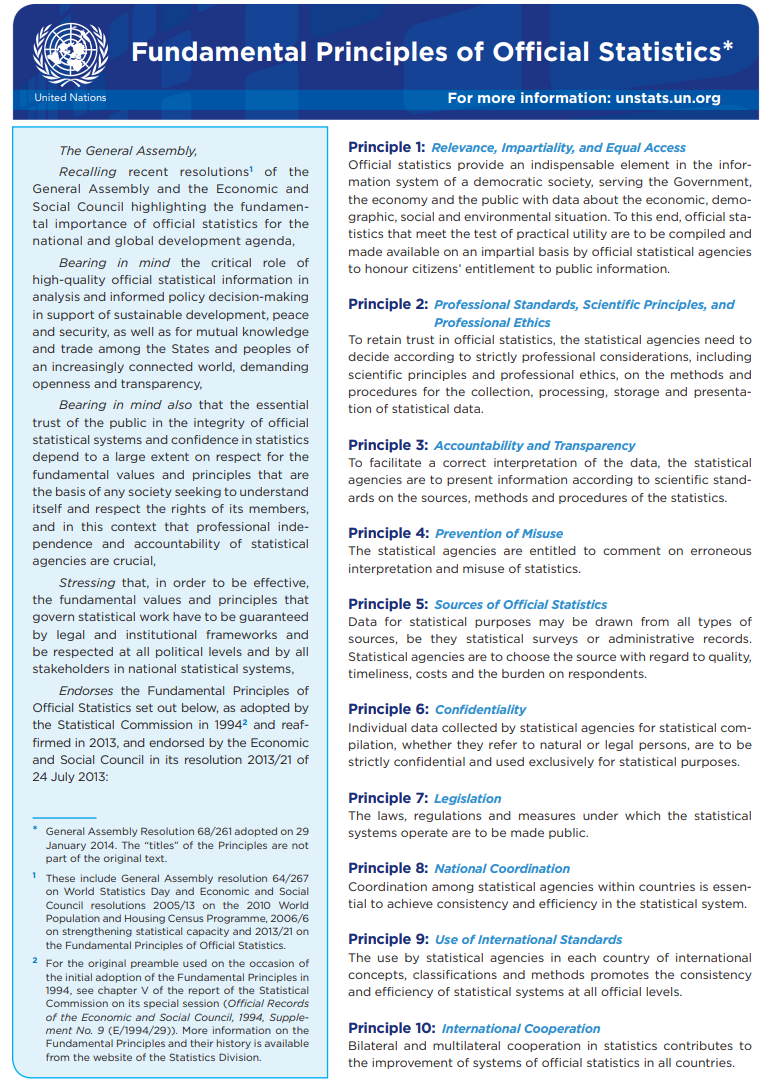
\includegraphics[width=\textwidth]{FundamentalPrinciplesOS.PNG}
    \end{column}
  \end{columns}
\end{frame}

\begin{frame}{Usual practice: Theory vs reality}
  \centering
  \includegraphics[width=0.9\textwidth]{ManualPipe1.png}

  \medskip

  \begin{itemize}
    \item Download some data and store it in an excel file
    \item Load the excel data into R to generate a chart
    \item Copy and paste the formatted table and chart into a word document and add some text and formatting to create the final report
  \end{itemize}
\end{frame}


\begin{frame}{Usual practice: In the end}
  \centering
  \includegraphics[width=0.9\textwidth]{ManualPipe1.png}

  \medskip

  In reality though, our ideal analytical pipeline can quickly become a complicated tangle of multiple file and data versions, programs, emails and final reports.
\end{frame}

\begin{frame}{What are the issues?}
  \begin{columns}[T]
    \begin{column}{0.5\textwidth}
      \begin{itemize}
        \item Lots of files
        \item Cut and paste is not a reliable, reproducible approach!
        \item Each operator has his/her own approach
        \item Several versions of code may coexist
        \item Mistakes hard to track
        \item The steps aren't recorded
        \item Testing is hard
        \item Reproducibility is not granted
        \item Quality is controlled only at the end
      \end{itemize}
    \end{column}
    \begin{column}{0.5\textwidth}
      
\includegraphics[width=\textwidth]{TraditionalMess.png}
      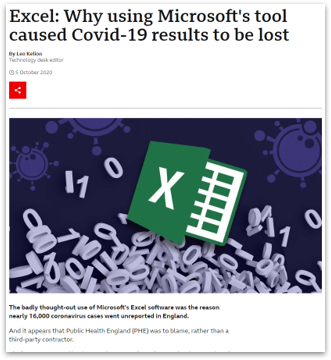
\includegraphics[width=\textwidth]{ExcelUK.png}
    \end{column}
  \end{columns}
\end{frame}

% Other slides go here...

\begin{frame}{What does a RAP look like?}
  \begin{columns}[T]
    \begin{column}{0.6\textwidth}
      \begin{itemize}
        \item It is a simple process:
          \begin{itemize}
            \item Linking inputs (data) to outputs (publication)
          \end{itemize}
      \end{itemize}
    \end{column}
    \begin{column}{0.4\textwidth}
      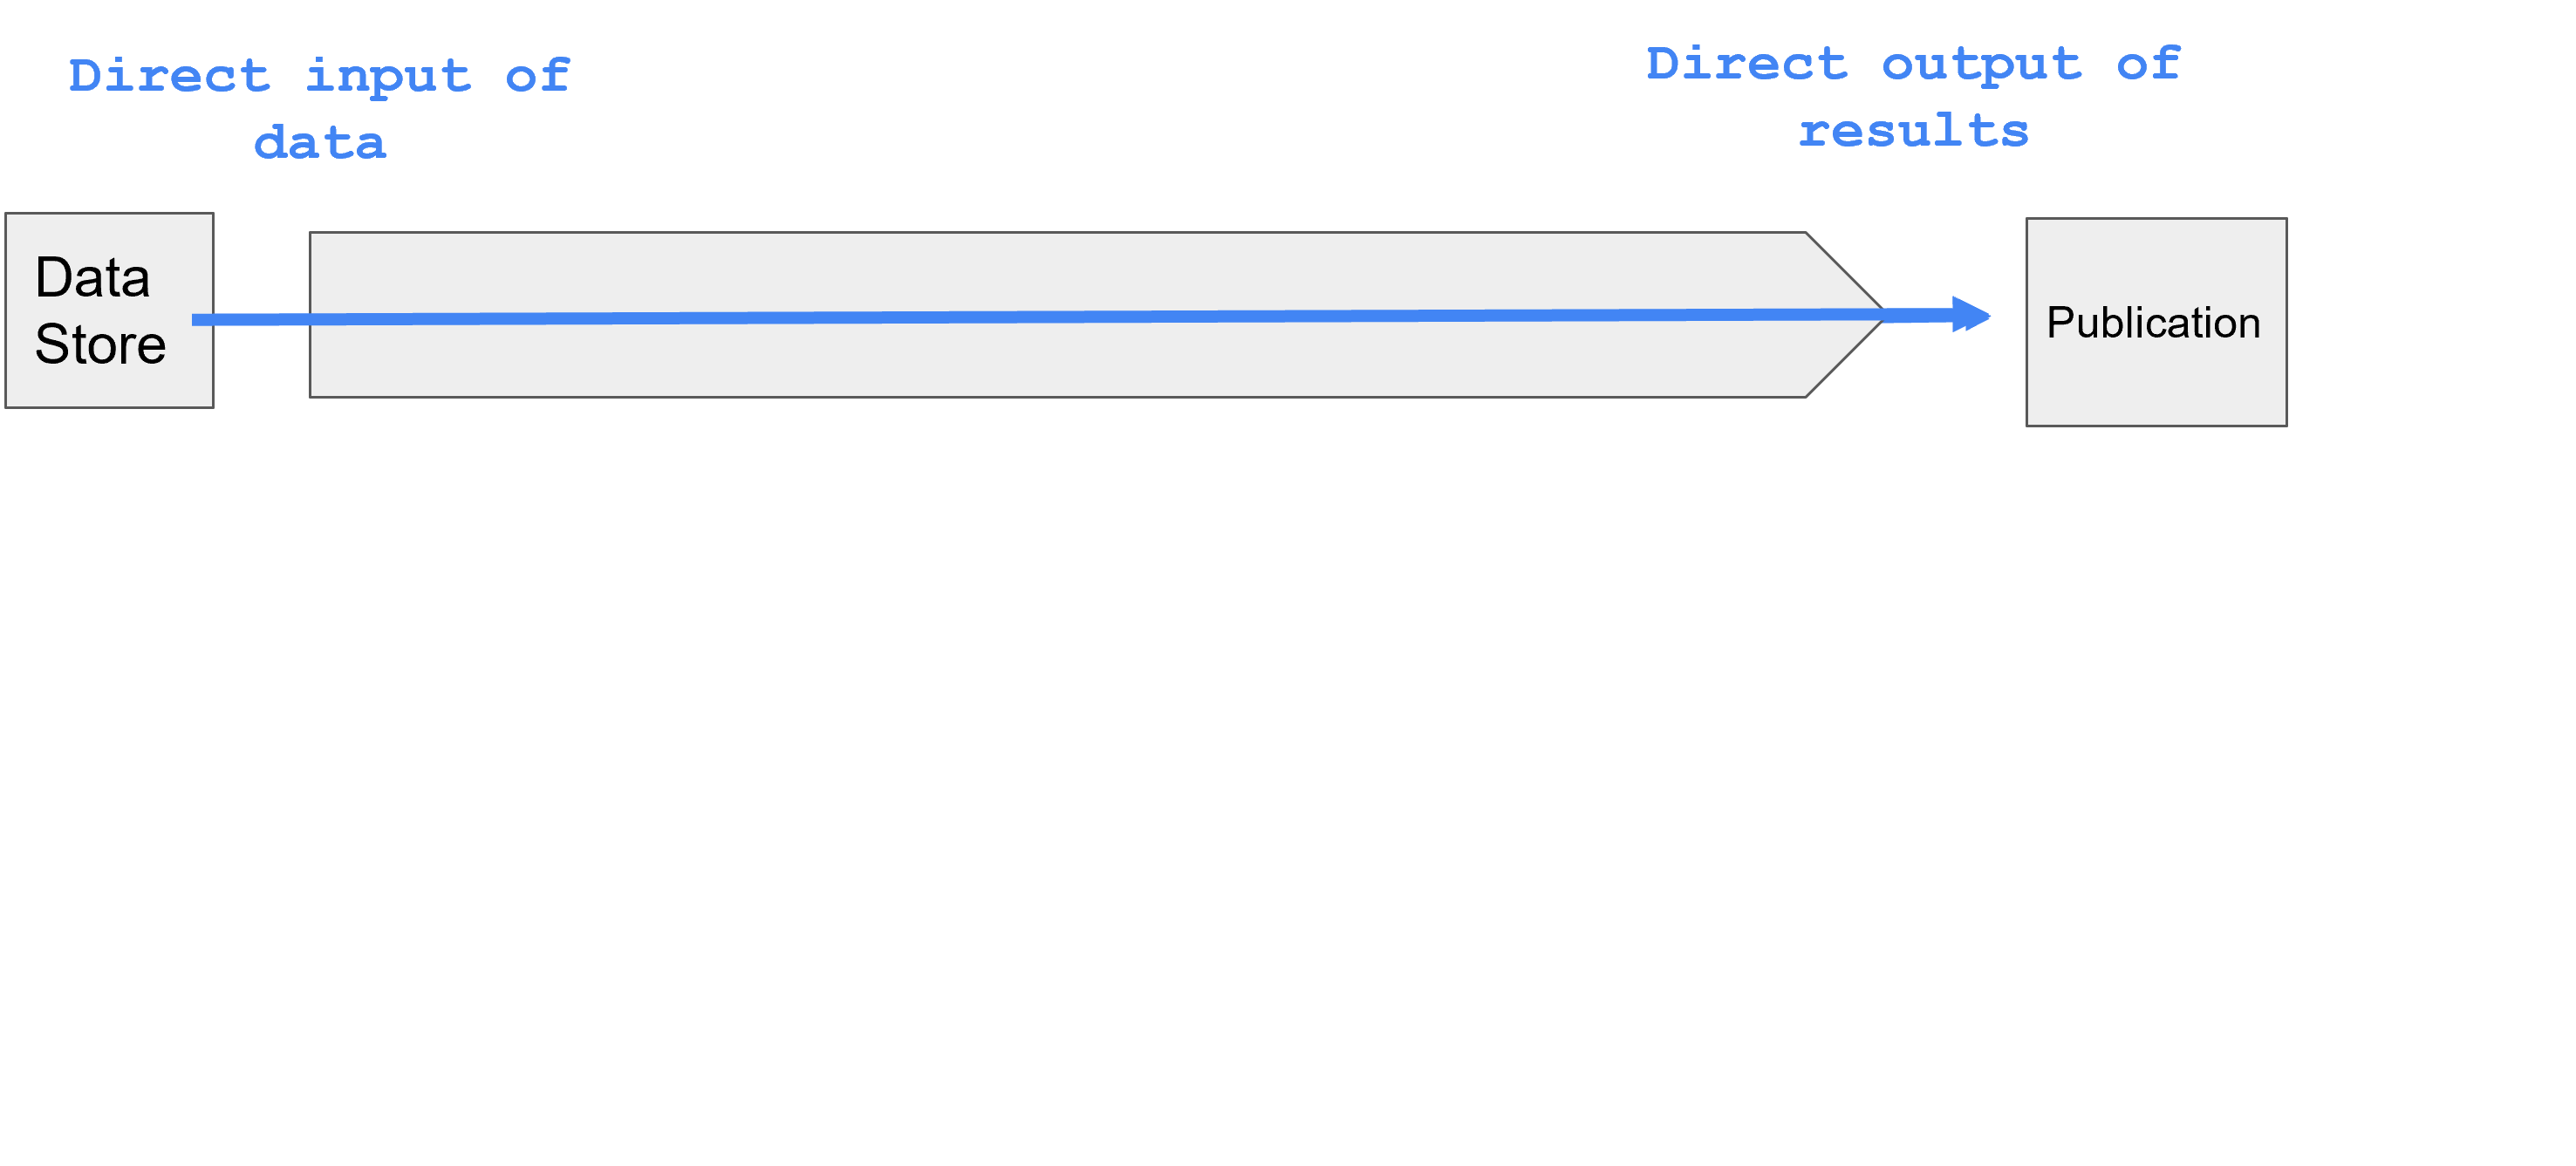
\includegraphics[width=\textwidth]{RAP-Pipeline1.png}
    \end{column}
  \end{columns}
\end{frame}

% Other slides go here...

\begin{frame}{Useful resources}
  \begin{itemize}
    \item The UK government RAP \href{https://ukgovdatascience.github.io/rap-website/index.html}{website}.
    \item UK best practice \href{https://gss.civilservice.gov.uk/policy-store/quality-statistics-in-government/\#reproducible-analytical-pipelines-rap-}{documentation}.
    \item A free RAP \href{https://www.udemy.com/course/reproducible-analytical-pipelines/}{course} to teach you all you need to know.
    \item How the Data Science Campus sets its coding \href{https://datasciencecampus.github.io/coding-standards/}{standards}.
    \item A new open-source \href{https://the-turing-way.netlify.com}{book} from the Alan Turing institute setting out how to do reproducible data science.
  \end{itemize}
\end{frame}

%\begin{frame}{Citing *The Turing Way*}
%  \justifying
%  \footnotesize
%  Many of the beautiful images used in this presentation were taken from *The Turing Way* book.
%
%  \medskip
%
%  Full citation:
%
%  *The Turing Way Community, Becky Arnold, Louise Bowler, Sarah Gibson, Patricia Herterich, Rosie Higman, ... Kirstie Whitaker. (2019, March 25). The Turing Way: A Handbook for Reproducible Data Science (Version v0.0.4). Zenodo. \url{http://doi.org/10.5281/zenodo.3233986}*
%\end{frame}



\end{document}


%%%%%%%%%%%%%%% Last Slide %%%%%%%%%%%%%%%%

\begin{frame}[allowframebreaks]%in case more than 1 slide needed
\frametitle{References}
    {\footnotesize
    %\bibliographystyle{authordate1}
    \bibliographystyle{apalike}
    \bibliography{c:/Chris/Visualisation/Visu}
    }
\end{frame}
\end{document}

%\bibliographystyle{authordate1}
%\bibliography{c:/Chris/Visualisation/Visu}
%\end{frame}

\begin{frame} % Cover slide
\frametitle{ }
\pause
 \begin{itemize}[<+->]
  \item[]
  \item
\end{itemize}
\end{frame}
